\section{Menu Phase: 2D Renderer}
With the VGA up and running and a robust double buffering system the game finally starts. The player enters the 2D renderer which displays the menu to setup the 3D game. It is pretty simple yet features a nice VGA trick where the four bank weak and cumbersome design turns into a strength.
\par
\begin{figure}[H]
\centering
\fullimage{first_menu.png}
\end{figure}
\par



Indeed with control over the bank mask, it is possible to write up to four pixels to the VRAM with only one write operation to the RAM! In the VGA layout below, you can see how pixels 0, 1, 2 and 3 are in different banks but at the same address (0x0000). By configuring the bank mask to 8+4+2+1 (15), it is possible to write to all banks simultaneously.\\
\par
\begin{figure}[H]
\centering
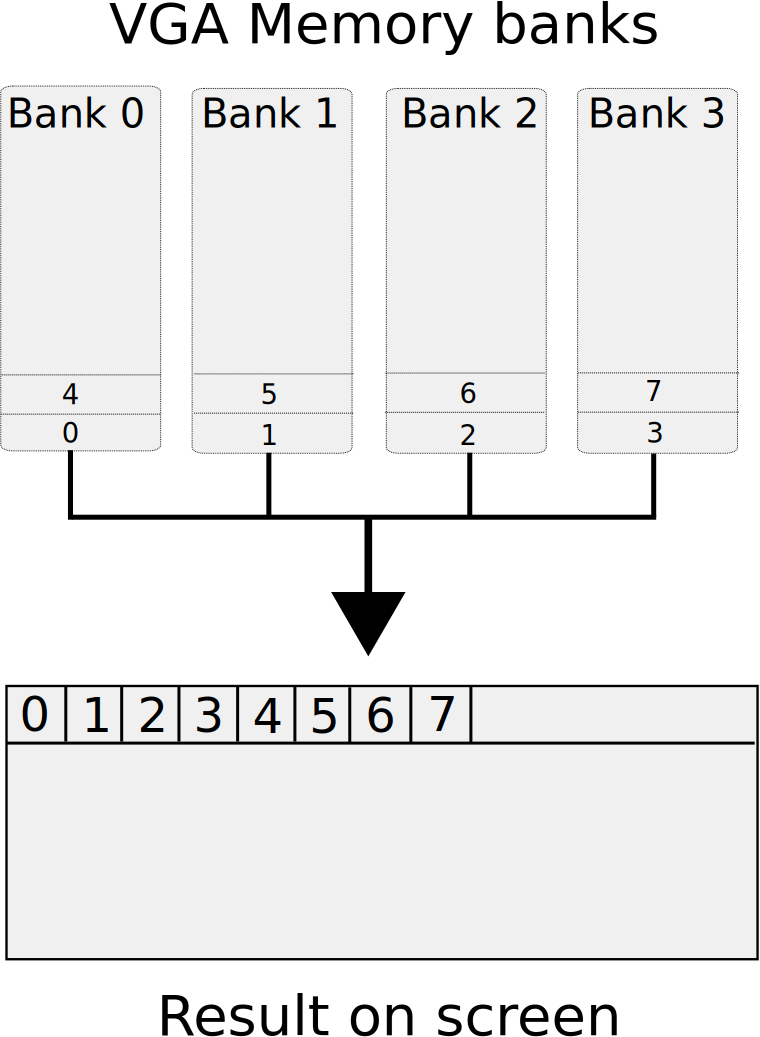
\includegraphics[width=0.6\textwidth]{imgs/drawings/vga_ram_screen_layout.pdf}
\end{figure}

\par
Therefore in order to clear the screen to red before drawing the menu, the 2D engine only performs 320x200/4 = 16,000 writes instead of 64,000. In the drawing above, pixels 0,1,2 and 3 would be written with one write operation. Then pixels 4,5,6 and 7 with an other write. And so on...\\

\par
\begin{minipage}{\textwidth}
\lstinputlisting[language=C]{code/vga_clear/optimal.c}
\end{minipage}
However there is a limitation to this trick: Only bytes at the same address in a bank can be written simultaneously. Pixel alignment with banks has to be carefully considered. Take the example of the following layout:\\
\par
\begin{figure}[H]
\centering
 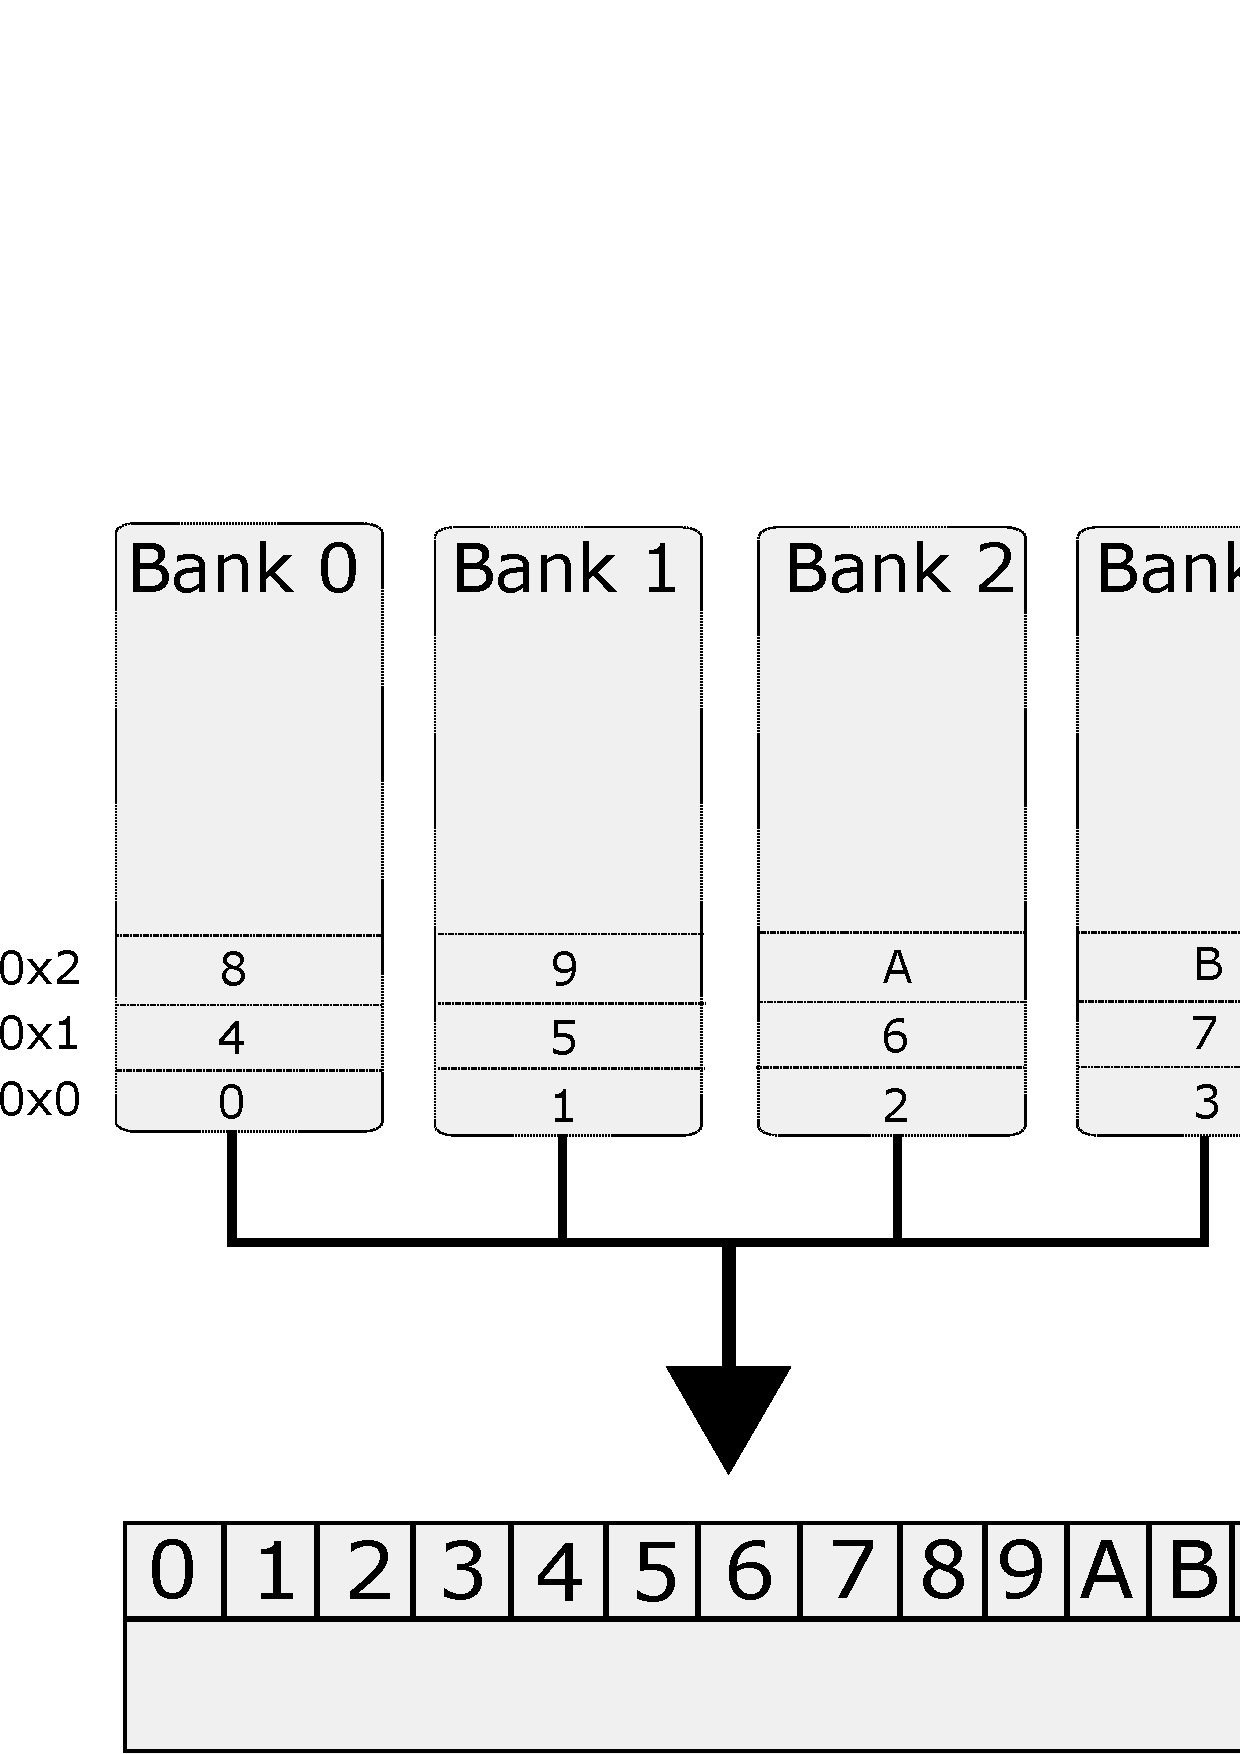
\includegraphics[width=.7\textwidth]{imgs/drawings/scalePost_explanation1.pdf}
 \end{figure}
Pixels 0, 1, 2, 3 can be written in one write.\\
Pixels 3 and 4 need two write operations.\\
Pixels 3, 4, 5, 6, 7, 8 would need three.\\


\par
The rest of the 2D renderer is pretty straight forward. It uses extensively the US Manager to render font and the Cache manager to retrieve the assets from HDD to the RAM. Note that Assets are called "pic" as opposed to "sprites" in 3D renderer. Pictures are all Huffman-compressed (VGADICT, VGAHEAD, VGAGRAPH). Menus are exactly what one would expect: Stored in an array of struct, featuring asset id and function pointers for each buttons. Here is the code to draw the "Main Menu" shown previously.\\

\par
\begin{minipage}{\textwidth}
\lstinputlisting[language=C]{code/menu.c}
\end{minipage}

\par
\begin{minipage}{\textwidth}
\lstinputlisting[language=C]{code/draw_main_menu.c}
\end{minipage}
\par
Notice how the \cw{C\_*} are macro defined in the files generated by \cw{IGRAB-ed}, the assets compiler.

